\documentclass[lettersize,journal]{IEEEtran}
\usepackage{amsmath,amsfonts}
\usepackage{algorithmic}
\usepackage{algorithm}
\usepackage{array}
\usepackage[caption=false,font=normalsize,labelfont=sf,textfont=sf]{subfig}
\usepackage{textcomp}
\usepackage{stfloats}
\usepackage{url}
\usepackage{verbatim}
\usepackage{graphicx}
\usepackage{cite}
\hyphenation{op-tical net-works semi-conduc-tor IEEE-Xplore}
% updated with editorial comments 8/9/2021

\begin{document}

\title{Bayesian Spatiotemporal Graph Neural Networks for Trustworthy Intrusion Detection in 5G/6G Networks}

\author{ Name,~\IEEEmembership{Student Member,~IEEE,}
         Name,~\IEEEmembership{Fellow,~IEEE}
        % <-this % stops a space
\thanks{This work was supported by [Funding Information].}% <-this % stops a space
\thanks{The authors are with [Your Institution], [City, Country] (e-mail: your.email@institution.edu).}
\thanks{Manuscript received [Date]; revised [Date].}}

% The paper headers
\markboth{IEEE Transactions on Information Forensics and Security,~Vol.~XX, No.~X, [Month]~2026}%
{Author \MakeLowercase{\textit{et al.}}: Bayesian Spatiotemporal Graph Neural Networks for Trustworthy Intrusion Detection}

\IEEEpubid{1556-6013~\copyright~2026 IEEE}
% Remember, if you use this you must call \IEEEpubidadjcol in the second
% column for its text to clear the IEEEpubid mark.

\maketitle

\begin{abstract}
The evolution toward 6G networks with AI-native architectures introduces new security challenges, where AI-driven intrusion detection systems (IDS) must not only achieve high accuracy but also provide trustworthy predictions with quantified uncertainty. Existing deep learning-based IDS often produce overconfident predictions on out-of-distribution samples and novel attacks, failing to meet the requirements of zero-trust architectures. This paper proposes BSTGCN, a Bayesian Spatiotemporal Graph Convolutional Network that integrates variational inference with packet-level spatiotemporal modeling for trustworthy network intrusion detection. BSTGCN constructs dynamic graphs over packet sequences using KNN-based similarity, captures temporal dependencies via Bayesian temporal convolutional networks (TCN), and models spatial relationships through Bayesian GraphSAGE, while quantifying epistemic and aleatoric uncertainty through Monte Carlo sampling. Evaluated on the 5G-NIDD dataset with 125,956 packet-window samples (50 packets/window, 23 features/packet) and 9 attack types, BSTGCN achieves 96.74\% accuracy and 91.65\% macro F1-score while providing uncertainty estimates that correlate with prediction errors (correlation: 0.118). The adaptive sampling strategy reduces validation time by 60\% while maintaining performance. BSTGCN demonstrates OOD detection capability, achieving AUROC of 0.823 under temporal distribution shift. In multi-hold-out evaluation across three diverse attack types (SlowrateDoS, SYNScan, ICMPFlood), BSTGCN achieves average AUROC of 0.878$\pm$0.04, outperforming STGCN+MC Dropout (0.856$\pm$0.04) and XGBoost+Entropy (0.812$\pm$0.05), while providing unique uncertainty decomposition capabilities. These results enable risk-aware security decisions, making BSTGCN suitable for deployment in 5G/6G zero-trust architectures.
\end{abstract}

\begin{IEEEkeywords}
Intrusion detection, Bayesian neural networks, graph neural networks, spatiotemporal modeling, uncertainty quantification, 5G/6G security, zero-trust architecture, trustworthy AI.
\end{IEEEkeywords}

\section{Introduction}
\IEEEPARstart{T}{he} evolution toward sixth-generation (6G) mobile networks is fundamentally reshaping the landscape of network security. According to the ITU-R IMT-2030 vision~\cite{ITU_IMT2030_2023} and IMT-2030(6G) Promotion Group white papers~\cite{IMT2030_6G_WhitePaper_2021}, 6G networks will adopt AI-native architectures where artificial intelligence (AI) is deeply integrated into wireless access, core networks, and edge computing layers. In this paradigm, AI transitions from an auxiliary tool for resource optimization to a core driver of network operations, undertaking critical security functions such as anomaly detection, threat identification, and risk assessment. However, this deep integration of AI introduces a new dimension of security risks: the trustworthiness of AI itself becomes a security concern.

\subsection{Motivation and Challenges}

Existing deep learning-based intrusion detection systems (IDS) have demonstrated impressive performance on benchmark datasets, achieving over 95\% accuracy on known attack types~\cite{Habeeb_NIDS_AI_Survey_2022,Rabiu_AIDriven_NIDS_Review_2025}. However, recent studies reveal a critical limitation: these models often produce overconfident predictions when facing zero-day attacks, attack variants, or distribution shifts~\cite{BCNN-IDS,Tabarisaadi2024}. This phenomenon arises from the inherent characteristics of deterministic neural networks, which forcibly map all inputs to known categories and output single-point predictions without expressing their internal epistemic uncertainty~\cite{Guo_Calibration_2017,Gal_Uncertainty_2016}. In preliminary experiments on the 5G-NIDD dataset, we observed that when using temporal splitting (training on the first 70\% time period, testing on the last 30\%), model accuracy dropped from 95\% to 88\%, while average confidence remained above 0.92. For rare attack types (comprising $<$2\% of samples), models achieved F1-scores below 70\% while maintaining average confidence of 0.85 on incorrect predictions. This ``high-confidence error'' phenomenon is particularly dangerous in security scenarios, as it can mislead security operators and result in false negatives.

This problem is especially acute in 6G network security scenarios, where security functions heavily rely on AI, making ``whether AI itself is trustworthy'' a new security concern. The core principle of zero-trust architecture (ZTA)~\cite{NIST-ZTA}---``never trust, always verify''---requires security decisions to meet the criteria of being ``explainable, measurable, and accountable.'' This imposes higher trustworthiness standards on AI-driven security systems~\cite{Afroogh2024TrustAI}. Specifically, trustworthy AI in 6G native network security should address four core dimensions: (1) \textbf{Quantifiable uncertainty}: models should output not only classification results but also confidence assessments of their predictions~\cite{Talpini2024}; (2) \textbf{Explainable decisions}: models should explain their judgments at the packet sequence or attack chain level~\cite{Mohale2025}; (3) \textbf{Cross-scenario generalization}: models should avoid overconfident judgments when facing temporal distribution drift or novel attack scenarios; (4) \textbf{Controllable behavior}: alert triggering behavior should be adjustable, allowing trade-offs between security and usability~\cite{Kim2024HumanInLoop}.

\subsection{Technical Gaps}

Network attacks exhibit structured patterns in both temporal and spatial dimensions. Temporally, attack behaviors manifest as correlated evolutionary patterns: port scans show incrementing port sequences, distributed denial-of-service (DDoS) attacks exhibit sudden traffic spikes, and slow-rate attacks display prolonged low-frequency anomalies. Spatially, similar attack packets form clustering structures in feature space: packets with the same protocol type, similar lengths, and identical transmission directions often belong to the same attack phase. However, existing intrusion detection methods face limitations in modeling these dual spatiotemporal dependencies.

Recurrent neural network (RNN) or Transformer-based temporal models focus on capturing sequential correlations in packet sequences but struggle to leverage spatial clustering information of similar packets. Graph neural network (GNN)-based methods~\cite{lo2022egraphsage,E-ResGAT,wang2025bsgat} can model network topology or traffic relationship graphs but often assume static structures, failing to adequately capture the temporal evolution of attacks. Recent spatiotemporal graph neural network approaches~\cite{EvolveGCN,TCG-IDS,PPT-GNN} have made progress but predominantly operate at host-level or flow-level granularity, requiring maintenance of flow state tables and pre-aggregated statistical features, facing computational complexity and memory overhead bottlenecks in high-concurrency scenarios~\cite{Pekar2021}.

More critically, existing methods almost universally adopt deterministic learning paradigms, with output ``probabilities'' being merely softmax-normalized results that do not reflect the model's true uncertainty~\cite{Guo_Calibration_2017}. This leads models to potentially produce high-confidence incorrect predictions when facing unknown attacks, distribution drift, or adversarial samples~\cite{BCNN-IDS,Tabarisaadi2024}, failing to meet the requirements of zero-trust architectures for trustworthy AI~\cite{NIST-ZTA}.

\subsection{Our Contributions}

To address these challenges, this paper proposes BSTGCN (Bayesian Spatiotemporal Graph Convolutional Network), a trustworthy intrusion detection framework that integrates Bayesian inference with packet-level spatiotemporal modeling. The main contributions are:

\begin{enumerate}
\item \textbf{Novel packet-level spatiotemporal graph modeling paradigm}: We propose a stateless packet-level modeling approach that uses Transformer encoders for global packet sequence encoding without maintaining per-flow state tables, constructs dynamic spatial graphs via KNN-based cosine similarity to capture similar packet clustering, and employs Bayesian spatiotemporal convolutional blocks to model temporal dependencies (causal dilated convolution) and spatial dependencies (GraphSAGE aggregation) in parallel, with gated fusion mechanisms to adaptively balance spatiotemporal features. This design maintains packet-level temporal resolution ($10^{-3}$ to $10^{-2}$ seconds) while avoiding the $O(M)$ overhead of flow table maintenance, making it suitable for high-concurrency 6G network scenarios.

\item \textbf{End-to-end Bayesian spatiotemporal graph neural network}: We introduce variational inference into spatiotemporal graph convolutional networks, modeling weight distributions through Bayesian linear layers to quantify epistemic uncertainty (model parameter uncertainty) and aleatoric uncertainty (data noise). We design an ELBO loss function with KL annealing strategy to avoid posterior collapse, and propose an adaptive Monte Carlo sampling strategy that reduces validation time by 60\% while maintaining performance, balancing uncertainty estimation accuracy and efficiency.

\item \textbf{Uncertainty-driven security decision support}: We deeply integrate uncertainty quantification with security operations workflows, designing alert prioritization mechanisms (risk scores based on prediction probability and uncertainty), human review strategies (triggering manual inspection for samples exceeding uncertainty thresholds), out-of-distribution (OOD) detection (identifying unknown attack types via high epistemic uncertainty), and active learning (selecting high-uncertainty samples for labeling and retraining). This transforms uncertainty from an ``internal model metric'' into ``actionable decision support.''

\item \textbf{Comprehensive evaluation on real 5G dataset}: We conduct systematic experiments on the 5G-NIDD dataset (125,956 packet-window samples, 50 packets/window, 23 optimized features/packet, 9 attack types), comparing against 10 baseline models including temporal models (CNN1D, GRU, TCN), non-temporal models (LightGBM, XGBoost), graph models (GCN, GAT), and spatiotemporal models (LSTM+GNN, Seq-STGCN, STGCN). BSTGCN achieves 96.74\% accuracy and 91.65\% macro F1-score, while providing uncertainty estimates that correlate with prediction errors (correlation: 0.118). The adaptive sampling strategy reduces validation time by 60\% while maintaining performance. BSTGCN demonstrates OOD detection capability through both temporal distribution shift (AUROC 0.823) and multi-hold-out evaluation across three diverse attack types (SlowrateDoS, SYNScan, ICMPFlood). In the latter, BSTGCN achieves average AUROC of 0.878$\pm$0.04, outperforming STGCN+MC Dropout (0.856$\pm$0.04) and XGBoost+Entropy (0.812$\pm$0.05), while providing unique uncertainty decomposition into epistemic and aleatoric components. This enables risk-aware alert prioritization, where processing the top 20\% of alerts covers 80\% of true attacks.
\end{enumerate}

The remainder of this paper is organized as follows: Section II reviews related work on spatiotemporal graph neural networks and Bayesian deep learning in intrusion detection. Section III presents the BSTGCN methodology, including problem formulation, architecture design, and training strategies. Section IV describes the experimental setup and datasets. Section V presents comprehensive results and analysis. Section VI discusses implications, limitations, and future work. Section VII concludes the paper.


\section{Related Work}

\subsection{Spatiotemporal Graph Neural Networks for Intrusion Detection}

With graph neural networks (GNN) demonstrating superior performance in structured data modeling, researchers have begun applying them to network intrusion detection, constructing spatiotemporal graphs that simultaneously capture communication structures and temporal evolution characteristics~\cite{Zhong_GNN_IDS_Survey_2024}. However, existing work varies in graph construction granularity and temporal modeling strategies, which affects detection granularity, response timeliness, and computational cost in practical deployment. To clarify the existing research landscape and highlight the modeling challenges in low-latency high-precision scenarios addressed by our work, we categorize related work into \textit{entity-centric methods} and \textit{traffic-centric methods}, with the latter further divided into \textit{flow-level} and \textit{packet-level} granularity.

\subsubsection{Entity-Centric Graph Modeling Methods}

Entity-centric methods use system entities such as hosts, users, files, and processes as graph nodes, constructing graph structures from security logs, alert events, or system call sequences to capture potential attack paths and behavior chains. Jiang et al.~\cite{jiang2020gnn} apply GCN on user behavior graphs for insider threat detection, significantly outperforming traditional machine learning methods. Kisanga et al.~\cite{kisanga2023graph} construct Activity-Event-Network (AEN) knowledge graphs and use GNN to classify anomalous events in DDoS and TOR traffic. Lakha et al.~\cite{lakha2023anomalous} combine GNN with Transformer to improve temporal modeling capability for intrusion detection. Sun et al.~\cite{sun2024gnnids} integrate attack graphs with host measurements to generate dynamic graphs, improving multi-stage attack detection effectiveness.

While entity graph modeling methods can improve attack chain identification and model interpretability, most rely on pre-constructed attack graphs or knowledge graphs with low update frequency, making them difficult to adapt to dynamically changing 5G environments. Moreover, these methods exhibit latency and insufficient granularity when processing raw network traffic.

\subsubsection{Traffic-Centric Graph Modeling Methods}

Traffic-centric spatiotemporal graph modeling methods can be further divided into flow-level and packet-level categories based on input granularity.

\paragraph{Flow-Level Graph Modeling Methods} These methods use NetFlow or bidirectional connection records as basic units, constructing static or dynamic host communication graphs based on communication parties, or treating each flow as a node to build flow-flow dependency graphs. E-GraphSAGE~\cite{lo2022egraphsage} represents IoT traffic as host communication graphs, using GraphSAGE to aggregate neighbor information for edge classification, achieving 2\% improvement in weighted F1-score over traditional machine learning on UNSW-NB15 and BoT-IoT datasets. E-ResGAT~\cite{E-ResGAT} converts network representations to line graphs where flows become nodes, applying attention mechanisms to aggregate two-hop neighborhoods. BS-GAT~\cite{wang2025bsgat} introduces graph attention networks to construct behavior similarity graphs, achieving 99\% binary classification F1-score. To capture temporal evolution, EvolveGCN~\cite{EvolveGCN} uses gated recurrent units (GRU) to update GCN weights over time, enabling the model to evolve with temporal dynamics. TCG-IDS~\cite{TCG-IDS} constructs dynamic graph sequences over time windows, employing Temporal Graph Networks (TGN)~\cite{TGN} encoders with triple contrastive learning strategies, achieving 99.48\% balanced accuracy on CSE-CIC-IDS2018. Lagraa et al.~\cite{lagraa2021botgm} propose BotGM, a port-interaction flow graph detection method achieving 95\% accuracy. Friji et al.~\cite{Friji2023} use graph convolution on flow dependency graphs to model attack paths, improving identification of concurrent/sequential attacks. Fu et al.~\cite{fu2023hypervision} construct flow interaction graphs combined with unsupervised graph embedding, performing well on encrypted traffic.

These methods typically rely on complete flow aggregation, requiring state table maintenance. In high-frequency, high-concurrency 5G access scenarios, they face detection latency and computational bottlenecks. Furthermore, their temporal dynamics modeling is often based on fixed sliding windows, making it difficult to capture sub-second behavioral evolution. More importantly, the dependency on flow tables means they inherently cannot perform stateless processing---a critical limitation for 5G scenarios where flow table maintenance overhead scales as $O(M)$ with $M$ concurrent flows~\cite{Pekar2021}, and where 80\% of flows contain fewer than 10 packets, leaving insufficient context for flow-based detection.

\paragraph{Packet-Level Graph Modeling Methods} Recent research has attempted to bypass the flow aggregation process, directly constructing graph structures on raw packet sequences to achieve lower-latency detection. Graph2vec+RF~\cite{Graph2vec+RF} constructs small-scale flow graphs based on the first several packets of each flow, using graph embedding and random forests for classification, achieving 96.99\% and 99.33\% accuracy on CIC-IDS2017 and CIC-IDS2018 respectively, validating the potential of ``few packets + graph modeling'' in early detection. GTAE-IDS~\cite{GTAE-IDS} models network flows as dynamic graphs using the first 2-8 packets, employing unsupervised graph Transformer autoencoders to extract global graph features, achieving over 98\% true positive rate with low false positives on CIC-IDS2018. PPT-GNN~\cite{PPT-GNN} constructs flow graph sequences within small time windows (0.5-5 seconds) at the NetFlow level, combining GNN with temporal convolution/recurrent structures, achieving 10.38\% improvement in multi-class F1-score over E-ResGAT and E-GraphSAGE through self-supervised pretraining.

Although these methods use packet-level data, it is important to note that they essentially still rely on flow extraction rather than strictly stateless processing. PPT-GNN, while using short windows and fewer packets, still depends on flow-level features and NetFlow generation processes---it replaces ``complete long flows'' with ``short time-window flow subsequences,'' remaining fundamentally flow-centric and stateful, not achieving true ``flow-table-free, stateless'' packet-level modeling. Overall, packet-level graph methods can capture fine-grained attack signals earlier, suitable for 5G scenarios requiring high temporal resolution and stateless modeling. However, current packet-level ST-GNN research remains sparse, with mainstream methods still flow-centric, limiting their timeliness and generalization capability.

\subsubsection{Comparison and Motivation}

In summary, entity graph methods emphasize global context and attack chain modeling, suitable for offline analysis, while traffic graph methods emphasize online detection and data-driven mining, more aligned with real-time security defense scenarios. Among traffic methods, flow-level approaches depend on state maintenance at the feature level, susceptible to short-flow proliferation and attacker evasion strategies. Packet-level graph modeling is still in early stages, with existing methods largely lacking graph-based temporal modeling capability and uncertainty characterization.

Despite the advances described above, existing spatiotemporal graph methods for intrusion detection share a fundamental limitation: \textit{they almost universally adopt deterministic learning paradigms}, with output ``probabilities'' being merely softmax-normalized results that do not reflect true model uncertainty~\cite{Guo_Calibration_2017}. This leads to potentially high-confidence incorrect predictions when facing unknown attacks, distribution drift, or adversarial samples, failing to meet zero-trust architecture requirements for trustworthy AI~\cite{NIST-ZTA}. To address these issues, we propose BSTGCN and BSTGNF models that construct dynamic graph sequences based on raw packets within sliding windows, combining heterogeneous graph attention mechanisms with variational Bayesian inference to achieve millisecond-level attack detection while quantifying model epistemic uncertainty, providing support for unknown attack rejection and interpretable decision-making.

\subsection{Bayesian Deep Learning in Security Scenarios}

Bayesian deep learning (BDL) introduces probability distributions over neural network weights, extending point estimates to distribution estimates to quantify predictive uncertainty~\cite{Gal_Uncertainty_2016}. Recent applications in network security have emerged but remain limited.

\textbf{Bayesian neural networks for intrusion detection}: BCNN-IDS~\cite{BCNN-IDS} applies Bayesian convolutional neural networks to NIDS, using variational inference and Monte Carlo Dropout to estimate weight posterior distributions, achieving high accuracy while providing uncertainty measures for each prediction on NSL-KDD and UNSW-NB15 datasets. BCNN-IDS distinguishes two types of uncertainty: \textit{epistemic uncertainty} (model uncertainty due to insufficient training data, reducible through more data or improved architectures) and \textit{aleatoric uncertainty} (inherent data noise, irreducible). This distinction is crucial for intrusion detection: high epistemic uncertainty suggests the model lacks experience with the sample, requiring human review or active learning; high aleatoric uncertainty indicates data noise or adversarial perturbations.

\textbf{Uncertainty-aware training and calibration}: Recent work focuses on improving models' uncertainty characterization. Tabarisaadi et al.~\cite{Tabarisaadi2024} propose uncertainty-aware training frameworks introducing multi-objective loss functions to simultaneously optimize prediction accuracy and uncertainty quality, adding KL divergence penalties to widen the gap between uncertainty distributions for correct and incorrect predictions. Li et al.~\cite{Li2025TrustworthyBayesian} construct a trustworthy Bayesian deep learning framework (TMFD) combining Bayesian neural networks with confidence calibration strategies, using $\alpha$-divergence variational inference for parameter posteriors and incorporating calibration error into loss functions (AMCL loss), significantly reducing expected calibration error (ECE).

\textbf{Bayesian graph neural networks}: While theoretical research on Bayesian GNNs has progressed, with frameworks like BGCN~\cite{Zhang2019BGCN} performing joint posterior inference over graph structure and GNN weights, and Graph DropConnect~\cite{Hasanzadeh2020GDC} using adaptive connection sampling to approximate Bayesian GNN training, few works have combined Bayesian inference with spatiotemporal graph modeling for network security. Existing Bayesian NIDS primarily focus on traditional flow statistical features or image-based traffic representations, unable to capture spatiotemporal dependencies and topological structures of network traffic.

\subsection{Research Gaps}

Synthesizing the above review, current research exhibits systematic gaps in uncertainty quantification for network intrusion detection: (1) \textbf{Insufficient structured modeling}: many Bayesian NIDS apply Bayesian neural networks only at the sample level, ignoring topological relationships between hosts and flows and temporal chains of attacks~\cite{BCNN-IDS}; (2) \textbf{Missing spatiotemporal dependency modeling}: existing Bayesian NIDS mainly focus on fixed-dimension flow feature vectors, unable to capture spatiotemporal dependencies~\cite{Tabarisaadi2024,Li2025TrustworthyBayesian}; (3) \textbf{Inadequate prior design}: most Bayesian deep models adopt default simple priors (e.g., independent Gaussian distributions), lacking integration of security domain prior knowledge~\cite{Wang2024KGetNID}; (4) \textbf{Disconnected explainability and uncertainty}: existing research often only provides uncertainty values without combining uncertainty information to explain model decisions or reveal anomaly causes.

This paper addresses these gaps by proposing BSTGCN, which integrates Bayesian inference with packet-level spatiotemporal graph modeling to achieve trustworthy intrusion detection with quantified uncertainty, explainable decisions, and cross-scenario generalization.

\section{Methodology}

\subsection{Problem Formulation}

We formulate network intrusion detection as a multi-class classification problem with uncertainty quantification. Given a short-term packet window of length $L$ extracted from raw network captures using a sliding window over global packet arrival order, where each packet is characterized by $D$ features, the input is $\mathbf{X} \in \mathbb{R}^{L \times D}$. Note that each window typically contains packets from multiple concurrent network flows, as packets are ordered by capture timestamp rather than grouped by flow identifiers. Our goal is to learn a probabilistic model $p(y|\mathbf{X}, \Theta)$ that predicts the dominant traffic scenario (attack type or benign) $y \in \{1, 2, \ldots, C\}$ (where $C=9$ includes benign traffic and 8 attack types) while quantifying the epistemic uncertainty arising from model parameters $\Theta$.

Unlike deterministic models that output a single prediction $\hat{y} = \arg\max_c p(y=c|\mathbf{X}, \hat{\Theta})$ with point-estimated parameters $\hat{\Theta}$, Bayesian models maintain a distribution over parameters $p(\Theta|\mathcal{D})$ given training data $\mathcal{D}$, enabling uncertainty quantification through the predictive distribution:
\begin{equation}
p(y|\mathbf{X}, \mathcal{D}) = \int p(y|\mathbf{X}, \Theta) p(\Theta|\mathcal{D}) d\Theta
\end{equation}

The integral in Eq.~(1) is analytically intractable for deep neural networks because: (a) the posterior distribution $p(\Theta|\mathcal{D})$ has no closed-form solution due to the complex, non-linear likelihood function induced by the network architecture; and (b) the high-dimensional parameter space (typically millions of parameters) makes exact integration computationally infeasible. To address these challenges, we employ variational inference to approximate the true posterior $p(\Theta|\mathcal{D})$ with a tractable variational distribution $q(\Theta)$ (typically factorized Gaussian), and then use Monte Carlo (MC) sampling to estimate the predictive distribution. Specifically, we draw $M$ parameter samples $\{\Theta^{(m)}\}_{m=1}^M$ from $q(\Theta)$ and compute:
\begin{equation}
p(y|\mathbf{X}, \mathcal{D}) \approx \frac{1}{M} \sum_{m=1}^M p(y|\mathbf{X}, \Theta^{(m)})
\end{equation}

This MC approximation has convergence rate $O(1/\sqrt{M})$ by the Central Limit Theorem, meaning that the estimation error decreases as we increase the number of samples. In our experiments, we use $M=20$ samples during inference, which provides a good balance between uncertainty estimation accuracy and computational efficiency. The variance of this predictive distribution across the $M$ forward passes serves as a measure of epistemic uncertainty, indicating the model's confidence in its prediction---high variance suggests that the model has seen few similar examples during training and is uncertain about the correct classification.

\subsection{BSTGCN Architecture}

Fig.~\ref{fig:architecture} illustrates the overall architecture of BSTGCN, which consists of four main components: (1) Transformer encoder for semantic representation, (2) KNN graph builder for dynamic graph construction, (3) stacked Bayesian spatiotemporal (ST) blocks for joint temporal-spatial modeling with uncertainty quantification, and (4) Bayesian aggregation and classifier for final prediction with epistemic uncertainty estimation via Monte Carlo (MC) sampling. The design philosophy is to keep computationally expensive components (Transformer encoder and KNN graph construction) deterministic while applying Bayesian inference to the ST blocks, aggregation, and classification layers where uncertainty quantification is most critical.

\begin{figure*}[!t]
\centering
\includegraphics[width=0.95\textwidth]{figures/bstgcn_architecture.png}
\caption{The overall architecture of BSTGCN. (Top) The main pipeline: input packet sequences are encoded by a Transformer encoder to obtain semantic representations, which are then used to construct a dynamic KNN graph. Three Bayesian ST blocks are stacked sequentially to progressively refine the representations. Bayesian aggregation pools node features via gated attention, and a Bayesian classifier outputs final predictions $\hat{y}$, probabilities $\hat{p}$, and epistemic uncertainty $\mathcal{U}_{\text{epi}}$ via MC sampling. (Bottom) Detail of a single Bayesian ST block: within each block, the temporal branch (Bayesian TCN with depthwise convolutions) and the spatial branch (Bayesian GraphSAGE with neighbor aggregation) process the input \textbf{in parallel}. Both branches sample weights from learned variational posteriors $\mathcal{N}(\mu, \sigma^2)$. A gated fusion mechanism with sigmoid gates adaptively combines the temporal features $H_t$ and spatial features $H_s$ to produce the output $H^{(\ell+1)}$.}
\label{fig:architecture}
\end{figure*}

\subsubsection{Transformer Encoder for Semantic Representation}

Given a batch of input packet sequences $\mathbf{X} \in \mathbb{R}^{B \times L \times D}$ (where $B$ is batch size, $L=50$ is sequence length, $D=25$ is feature dimension), we first apply a linear projection followed by a lightweight Transformer encoder (1 layer, 8 attention heads) to capture global dependencies across the packet sequence and obtain semantic representations:
\begin{equation}
\mathbf{X}' = \text{TransformerEncoder}(\text{Linear}(\mathbf{X})) \in \mathbb{R}^{B \times L \times d_h}
\end{equation}
where $d_h=128$ is the hidden dimension. The Transformer encoder enriches each packet representation with contextual information from the entire sequence through self-attention. This component is kept deterministic because: (a) self-attention computation is already expensive ($O(L^2 d_h)$), and Bayesian variants would multiply this cost by the number of MC samples; (b) the Transformer primarily serves feature extraction, and uncertainty in this stage has limited impact on final predictions.

\subsubsection{KNN Graph Builder}

To model spatial relationships between packets, we construct a dynamic K-nearest neighbor (KNN) graph based on cosine similarity in the learned representation space. As shown in Fig.~\ref{fig:architecture}, the KNN Graph Builder takes the semantic features $\mathbf{X}'$ as input and outputs an adjacency matrix $\mathbf{A}$. For each sample in the batch, we compute pairwise cosine similarities:
\begin{equation}
\text{sim}(\mathbf{x}'_i, \mathbf{x}'_j) = \frac{\mathbf{x}'_i \cdot \mathbf{x}'_j}{\|\mathbf{x}'_i\| \|\mathbf{x}'_j\|}
\end{equation}

The adjacency matrix $\mathbf{A} \in \mathbb{R}^{B \times L \times L}$ is constructed by connecting each packet to its $k=10$ nearest neighbors:
\begin{equation}
\mathbf{A}_{ij} = \begin{cases}
1, & \text{if } j \in \text{TopK}(\text{sim}(\mathbf{x}'_i, \mathbf{x}'_j), k) \\
0, & \text{otherwise}
\end{cases}
\end{equation}

The adjacency matrix is then symmetrized: $\mathbf{A} \leftarrow (\mathbf{A} + \mathbf{A}^\top) / 2$. This KNN graph captures spatial clustering: similar packets (e.g., same protocol, similar length) are connected, enabling message passing to aggregate information from related packets. Graph construction is kept deterministic because: (a) KNN search is computationally intensive, and sampling multiple graph structures would be prohibitively expensive; (b) the Bayesian ST blocks will model uncertainty in how information flows through this fixed structure.

\subsubsection{Bayesian Spatiotemporal Blocks}

As shown in the bottom panel of Fig.~\ref{fig:architecture}, the core of BSTGCN consists of $N=3$ stacked Bayesian spatiotemporal (ST) blocks. Each block takes the hidden representation $\mathbf{H}^{(\ell)}$ and the adjacency matrix $\mathbf{A}$ as inputs, and contains two parallel branches---a temporal branch and a spatial branch---followed by a gated fusion mechanism.

\textbf{Temporal Branch (Bayesian TCN)}: The temporal branch employs Bayesian TCN with detailed depthwise separable convolutions to capture temporal dependencies. For the $\ell$-th ST block with dilation rate $d_\ell = 2^{\ell-1}$ (i.e., $\{1, 2, 4\}$ for three blocks), the temporal branch computes:
\begin{equation}
\mathbf{H}_t = \text{BayesianTCN}(\mathbf{H}^{(\ell-1)}), \quad \mathbf{W}_t \sim \mathcal{N}(\boldsymbol{\mu}, \boldsymbol{\sigma}_t^2)
\end{equation}

The Bayesian TCN consists of depthwise convolution (applying a separate filter to each channel) followed by pointwise convolution ($1\times1$ convolution for channel mixing). All convolution layers use Bayesian weights sampled from learned variational posteriors $q(\mathbf{W}_t) = \mathcal{N}(\boldsymbol{\mu}, \text{diag}(\boldsymbol{\sigma}_t^2))$. During forward propagation, weights are sampled using the reparameterization trick:
\begin{equation}
\mathbf{W}_t = \boldsymbol{\mu} + \boldsymbol{\sigma}_t \odot \boldsymbol{\epsilon}, \quad \boldsymbol{\epsilon} \sim \mathcal{N}(0, \mathbf{I})
\end{equation}

The dilated causal convolutions ensure that the receptive field grows exponentially with depth, covering approximately 20 packets across three blocks, enabling the model to capture both short-term and long-term temporal patterns.

\textbf{Spatial Branch (Bayesian GraphSAGE)}: The spatial branch employs Bayesian GraphSAGE with neighbor aggregation to model spatial dependencies based on the KNN graph structure. For each packet node $i$, we aggregate information from its neighbors $\mathcal{N}(i)$ defined by the adjacency matrix $\mathbf{A}$:
\begin{align}
\mathbf{h}_{\text{neigh}} &= \frac{1}{|\mathcal{N}(i)|} \sum_{j \in \mathcal{N}(i)} \mathbf{h}_j^{(\ell-1)} \\
\mathbf{H}_s &= \sigma\left( \mathbf{W}_{\text{self}} \mathbf{H}^{(\ell-1)} + \mathbf{W}_{\text{neigh}} \mathbf{H}_{\text{neigh}} \right), \quad \mathbf{W}_s \sim \mathcal{N}(\boldsymbol{\mu}, \boldsymbol{\sigma}_s^2)
\end{align}
where $\mathbf{W}_{\text{self}}$ and $\mathbf{W}_{\text{neigh}}$ are Bayesian linear layers with variational posteriors, and $\sigma$ denotes the GELU activation function. Similar to the temporal branch, weights are sampled from $q(\mathbf{W}_s) = \mathcal{N}(\boldsymbol{\mu}, \text{diag}(\boldsymbol{\sigma}_s^2))$.

We choose GraphSAGE over attention-based methods (e.g., GATv2) for efficiency: GraphSAGE's neighbor aggregation has linear complexity $O(L \cdot k \cdot d_h)$, while attention mechanisms have quadratic complexity $O(L^2 \cdot d_h)$. Since the KNN graph already selects the most relevant neighbors, the additional expressiveness of attention provides diminishing returns while significantly increasing computational cost.

\textbf{Gated Fusion}: As illustrated in Fig.~\ref{fig:architecture}, the gated fusion mechanism adaptively balances temporal and spatial information. Given temporal branch output $\mathbf{H}_t$ and spatial branch output $\mathbf{H}_s$, we compute adaptive gates using sigmoid activation:
\begin{align}
g_t &= \text{Sigmoid}(\text{Linear}_t(\mathbf{H}^{(\ell-1)})) \\
g_s &= \text{Sigmoid}(\text{Linear}_s(\mathbf{H}^{(\ell-1)}))
\end{align}

The gates are normalized to sum to 1:
\begin{equation}
g_t \leftarrow \frac{g_t}{g_t + g_s + \epsilon}, \quad g_s \leftarrow \frac{g_s}{g_t + g_s + \epsilon}
\end{equation}
where $\epsilon=10^{-8}$ ensures numerical stability. The fused output combines both branches with residual connection:
\begin{equation}
\mathbf{H}^{(\ell+1)} = \text{LayerNorm}(g_t \odot \mathbf{H}_t + g_s \odot \mathbf{H}_s + \mathbf{H}^{(\ell)})
\end{equation}

The residual connection and layer normalization stabilize training and enable gradient flow through deep networks.





\subsubsection{Bayesian Aggregation and Classification}

As shown in Fig.~\ref{fig:architecture}, after processing through $N=3$ ST blocks, the enriched packet representations $\mathbf{H}^{(N)} \in \mathbb{R}^{B \times L \times d_h}$ are aggregated and classified through two Bayesian components.

\textbf{Bayesian Aggregation (Gated Attention Pooling)}: To obtain a window-level (graph-level) representation for classification, we employ a Bayesian gated attention pooling mechanism:
\begin{align}
\mathbf{a} &= \text{softmax}(\text{BayesianLinear}(\mathbf{H}^{(N)})) \in \mathbb{R}^{B \times L} \\
\mathbf{h}_{\text{graph}} &= \sum_{i=1}^L a_i \mathbf{h}_i^{(N)} \in \mathbb{R}^{B \times d_h}
\end{align}

The attention weights $\mathbf{a}$ are learned through a Bayesian linear layer, allowing the model to express uncertainty about which packets are most informative for classification.

\textbf{Bayesian Classifier}: The aggregated graph representation is then passed through a two-layer Bayesian classifier:
\begin{align}
\mathbf{z} &= \text{LayerNorm}(\text{GELU}(\text{BayesianLinear}_1(\mathbf{h}_{\text{graph}}))) \in \mathbb{R}^{B \times d_h/2} \\
\mathbf{logits} &= \text{BayesianLinear}_2(\mathbf{z}) \in \mathbb{R}^{B \times C}
\end{align}

The class probabilities are obtained via softmax: $p(y=c|\mathbf{X}, \Theta) = \text{softmax}(\mathbf{logits})_c$.

\textbf{Inference via MC Sampling}: As illustrated in Fig.~\ref{fig:architecture}, during inference, we perform Monte Carlo (MC) sampling to obtain the final prediction $\hat{y}$, class probabilities $\hat{p}$, and epistemic uncertainty $\mathcal{U}_{\text{epi}}$. By drawing $M$ weight samples from the variational posteriors $q(\mathbf{W})$ across all Bayesian layers, we compute the predictive distribution and quantify epistemic uncertainty through mutual information. The detailed uncertainty quantification procedure is described in Section~\ref{sec:uncertainty}.

\subsection{Variational Inference and Training}

\subsubsection{ELBO Loss Function}

We train BSTGCN by maximizing the evidence lower bound (ELBO), which decomposes into a reconstruction term (classification loss) and a KL divergence term (regularization):
\begin{equation}
\mathcal{L}_{\text{ELBO}} = \mathbb{E}_{q(\Theta)}[\log p(\mathcal{D}|\Theta)] - \beta \cdot \text{KL}[q(\Theta) \| p(\Theta)]
\end{equation}

The reconstruction term is the expected log-likelihood of the training data under the variational posterior. We use label-smoothed cross-entropy loss:
\begin{equation}
\mathcal{L}_{\text{recon}} = -\frac{1}{N} \sum_{i=1}^N \sum_{c=1}^C \tilde{y}_{ic} \log p(y_i=c|\mathbf{x}_i, \Theta)
\end{equation}
where $\tilde{y}_{ic} = (1-\alpha) y_{ic} + \alpha / C$ with smoothing factor $\alpha=0.1$. Label smoothing prevents the model from becoming overconfident and improves generalization.

The KL divergence term measures the discrepancy between the variational posterior $q(\Theta)$ and the prior $p(\Theta)$. For Gaussian priors $p(\mathbf{W}) = \mathcal{N}(0, \sigma_{\text{prior}}^2 \mathbf{I})$ and Gaussian variational posteriors $q(\mathbf{W}) = \mathcal{N}(\boldsymbol{\mu}_W, \text{diag}(\boldsymbol{\sigma}_W^2))$, the KL divergence has a closed-form solution:
\begin{equation}
\text{KL} = \frac{1}{2} \sum_{i,j} \left[ \frac{\sigma_{W,ij}^2}{\sigma_{\text{prior}}^2} + \frac{\mu_{W,ij}^2}{\sigma_{\text{prior}}^2} - 1 - 2\log\frac{\sigma_{W,ij}}{\sigma_{\text{prior}}} \right]
\end{equation}

The total KL divergence is summed over all Bayesian layers in the network.

\subsubsection{KL Annealing Strategy}

Directly optimizing the ELBO can lead to posterior collapse, where the KL term dominates early in training, causing the variational posterior to collapse to the prior and preventing the model from learning meaningful representations. To address this, we employ a KL annealing strategy:
\begin{equation}
\mathcal{L} = \mathcal{L}_{\text{recon}} + \beta(t) \cdot \text{KL}, \quad \beta(t) = \beta_{\max} \cdot \min\left(1, \frac{t}{T_{\text{warmup}}}\right)
\end{equation}
where $\beta_{\max}=1.5\times10^{-4}$, $T_{\text{warmup}}=40$ epochs, and $t$ is the current epoch. During the warmup phase ($t < T_{\text{warmup}}$), $\beta(t)$ gradually increases from 0 to $\beta_{\max}$, allowing the model to first learn to classify accurately before regularizing the posterior.

\subsubsection{Optimization and Regularization}

We use the AdamW optimizer with learning rate $\eta=5\times10^{-4}$ and weight decay $\lambda=10^{-4}$. The learning rate follows a cosine annealing schedule with 10-epoch warmup and maximum 150 epochs. Gradient clipping with maximum norm 0.5 prevents exploding gradients. We apply dropout with rate 0.15 after each activation function for additional regularization.

To address class imbalance in the 5G-NIDD dataset, we use inverse frequency weighting: $w_c = N / (C \cdot N_c)$, where $N$ is the total number of samples, $C=9$ is the number of classes, and $N_c$ is the number of samples in class $c$. For extremely rare classes (e.g., ICMPFlood with only 173 samples), we apply additional weight boosting.

\subsection{Uncertainty Quantification}
\label{sec:uncertainty}

\subsubsection{Monte Carlo Sampling}

At inference time, we quantify predictive uncertainty through Monte Carlo (MC) sampling. For each input $\mathbf{X}$, we draw $M$ parameter samples from the variational posterior $q(\Theta)$ and compute $M$ predictions:
\begin{equation}
\Theta^{(m)} \sim q(\Theta), \quad p^{(m)} = p(y|\mathbf{X}, \Theta^{(m)}), \quad m=1,\ldots,M
\end{equation}

The predictive distribution is approximated by the empirical average:
\begin{equation}
\bar{p}_c = \frac{1}{M} \sum_{m=1}^M p_c^{(m)}, \quad c=1,\ldots,C
\end{equation}

The final prediction is $\hat{y} = \arg\max_c \bar{p}_c$.

\subsubsection{Epistemic Uncertainty via Mutual Information}

We quantify epistemic uncertainty (model uncertainty) using mutual information between predictions and model parameters:
\begin{equation}
\mathcal{U}_{\text{epi}}(\mathbf{X}) = \mathcal{H}\left[\mathbb{E}_{\Theta}[p(y|\mathbf{X},\Theta)]\right] - \mathbb{E}_{\Theta}\left[\mathcal{H}[p(y|\mathbf{X},\Theta)]\right]
\end{equation}
where $\mathcal{H}[p] = -\sum_c p_c \log p_c$ is the entropy. The first term measures the entropy of the average prediction (total uncertainty), while the second term measures the average entropy of individual predictions (aleatoric uncertainty). Their difference captures epistemic uncertainty: high values indicate that different parameter samples produce divergent predictions, suggesting the model is uncertain about the input.

In practice, we compute:
\begin{align}
\mathcal{U}_{\text{epi}} &= -\sum_c \bar{p}_c \log \bar{p}_c + \frac{1}{M} \sum_{m=1}^M \sum_c p_c^{(m)} \log p_c^{(m)}
\end{align}

We use PyTorch's \texttt{torch.special.entr} function to handle the case $p=0$ gracefully.

\subsubsection{Adaptive Monte Carlo Sampling}

Standard MC inference requires a fixed number of samples (e.g., $M=30$), which can be computationally expensive. We propose an adaptive sampling strategy that adjusts the number of samples based on the model's confidence:

\begin{algorithm}[H]
\caption{Adaptive Monte Carlo Sampling}
\label{alg:adaptive_mc}
\begin{algorithmic}[1]
\STATE Initialize $M_{\min}=3$, $M_{\max}=30$, $\tau_{\text{conf}}=0.95$, $\tau_{\text{unc}}=0.05$
\STATE Sample $M_{\min}$ times and compute $\bar{p}$ and $\mathcal{U}_{\text{epi}}$
\IF{$\max_c \bar{p}_c > \tau_{\text{conf}}$ \AND $\mathcal{U}_{\text{epi}} < \tau_{\text{unc}}$}
    \STATE \textbf{return} $\bar{p}$, $\mathcal{U}_{\text{epi}}$ \quad // High confidence, low uncertainty
\ELSE
    \STATE Continue sampling up to $M_{\max}$
    \STATE Recompute $\bar{p}$ and $\mathcal{U}_{\text{epi}}$ with all samples
    \STATE \textbf{return} $\bar{p}$, $\mathcal{U}_{\text{epi}}$
\ENDIF
\end{algorithmic}
\end{algorithm}

For samples where the model is highly confident and uncertainty is low (e.g., typical benign traffic), 3 samples suffice. For uncertain samples (e.g., boundary cases, novel attacks), we use the full 30 samples to accurately estimate uncertainty. This strategy reduces validation time by approximately 60\% while maintaining classification performance.

\subsubsection{Temperature Scaling for Calibration}

MC-averaged predictions from Bayesian neural networks tend to be underconfident (conservative) because averaging over multiple weight samples produces flatter probability distributions compared to deterministic softmax outputs. To improve calibration, we apply temperature scaling~\cite{Guo_Calibration_2017} as a post-processing step:
\begin{equation}
\bar{p}_c^{\text{scaled}} = \frac{\exp(\log \bar{p}_c / T)}{\sum_{c'} \exp(\log \bar{p}_{c'} / T)}
\end{equation}
where $T$ is a temperature parameter learned on the validation set by minimizing negative log-likelihood. A temperature $T < 1$ sharpens the probability distribution, increasing confidence for the predicted class. This simple calibration technique preserves the uncertainty information from MC sampling while aligning predicted probabilities with actual accuracy, achieving well-calibrated predictions suitable for risk-based decision-making.

\subsubsection{Deep Ensemble for Enhanced OOD Detection}

While a single BSTGCN model provides uncertainty estimates through MC sampling over weight distributions, we further improve out-of-distribution (OOD) detection by employing a Deep Ensemble strategy~\cite{Lakshminarayanan2017Ensemble}. Deep Ensembles train multiple independent models with different random initializations, capturing diverse modes of the posterior distribution that a single model may miss.

Given $K$ independently trained BSTGCN models $\{f_1, \ldots, f_K\}$, each initialized with a different random seed, we perform ensemble inference as follows:
\begin{enumerate}
\item For each model $f_k$, perform $M$ MC samples to obtain predictions $\{p_k^{(m)}\}_{m=1}^M$
\item Compute the model-level average: $\bar{p}_k = \frac{1}{M} \sum_{m=1}^M p_k^{(m)}$
\item Compute the ensemble average: $\bar{p}_{\text{ens}} = \frac{1}{K} \sum_{k=1}^K \bar{p}_k$
\end{enumerate}

The epistemic uncertainty is computed using mutual information over the ensemble:
\begin{equation}
\mathcal{U}_{\text{epi}}^{\text{ens}} = \mathcal{H}[\bar{p}_{\text{ens}}] - \frac{1}{K} \sum_{k=1}^K \mathcal{H}[\bar{p}_k]
\end{equation}

This formulation captures two sources of epistemic uncertainty: (1) within-model uncertainty from MC sampling over weight distributions, and (2) between-model uncertainty from different random initializations. The combination provides more robust uncertainty estimates, particularly for OOD samples where different models may disagree significantly.

In our experiments, we use $K=7$ models and $M=50$ MC samples per model. The ensemble can further improve OOD detection beyond single-model BSTGCN (average AUROC 0.878) at the cost of 7$\times$ training time and $K \times M$ forward passes during inference.

\section{Experimental Setup}

\subsection{Dataset}

We evaluate BSTGCN on the 5G-NIDD (5G Network Intrusion Detection Dataset), which contains real traffic collected from two 5G base stations. The dataset comprises 1,215,890 flow records covering 1 benign class and 8 attack types. Instead of using pre-aggregated flow-level statistics, we directly process raw pcapng capture files to preserve fine-grained packet-level information. Table~\ref{tab:dataset} shows the class distribution at both flow and packet levels.

\begin{table}[!t]
\caption{5G-NIDD Dataset: Flow vs. Packet Distribution\label{tab:dataset}}
\centering
\setlength{\tabcolsep}{3pt}
\begin{tabular}{lrrrr}
\hline
\textbf{Class} & \textbf{Flows} & \textbf{\%} & \textbf{Packets} & \textbf{\%} \\
\hline
UDPFlood & 456,168 & 37.5 & 1,871,358 & 34.89 \\
HTTPFlood & 139,827 & 11.5 & 1,361,748 & 25.39 \\
ICMPFlood & 1,155 & 0.1 & 607,661 & 11.33 \\
SlowrateDoS & 72,953 & 6.0 & 539,489 & 10.06 \\
SYNFlood & 9,727 & 0.8 & 446,004 & 8.32 \\
TCPConnectScan & 19,454 & 1.6 & 193,353 & 3.61 \\
UDPScan & 15,807 & 1.3 & 177,034 & 3.30 \\
SYNScan & 19,454 & 1.6 & 146,581 & 2.73 \\
Benign & 498,752 & 41.0 & 20,086 & 0.37 \\
\hline
\textbf{Total} & \textbf{1,215,890} & \textbf{100} & \textbf{5,363,314} & \textbf{100} \\
\hline
\end{tabular}
\end{table}

A striking observation from Table~\ref{tab:dataset} is the distribution discrepancy between flows and packets: Benign traffic accounts for 41.0\% of flows but only 0.37\% of packets, because benign SSH sessions consist of short-lived interactive flows ($\sim$0.04 packets/flow) while attack traffic generates far more packets per flow (ICMPFlood: $\sim$526 packets/flow). The packet-level distribution more accurately reflects actual network load, motivating our packet-based approach. Flow-based detection introduces two limitations: (1) \textit{detection latency}---waiting for flow termination; (2) \textit{state overhead}---maintaining per-flow state tables. Our sliding window approach enables real-time detection without flow reconstruction.

\noindent Packets are organized by global capture timestamp (not grouped by flow), and we apply a sliding window to construct samples. For each pcapng file containing $N$ packets, we extract samples using:
\begin{equation}
\text{num\_samples} = \left\lfloor \frac{N - L}{s} \right\rfloor + 1
\end{equation}
where $L$ is the window length (packets per sample) and $s$ is the stride. Each window contains packets from multiple concurrent network flows, representing a short-term traffic snapshot.

\textbf{Feature engineering}: Each packet is characterized by 23 optimized features: (1) \textit{temporal}: relative timestamp within the window; (2) \textit{size}: packet length; (3) \textit{protocol}: TCP/UDP/ICMP indicator; (4) \textit{IP addresses}: source and destination IPs encoded as 4 separate bytes (0-255 range each) instead of 32-bit integers to ensure uniform feature scaling; (5) \textit{ports}: source and destination port numbers; (6) \textit{IP header}: TTL, ToS, flags; (7) \textit{TCP header}: SYN/ACK/PSH flags, window size, sequence and acknowledgment numbers (modulo $10^6$); (8) \textit{ICMP}: type field. This 23-dimensional feature set was derived through variance analysis and redundancy elimination from an initial 25-dimensional set, removing near-constant features (e.g., icmp\_code with std=0.04) and redundant features (e.g., ip\_len highly correlated with packet\_length).

\textbf{Window configuration}: We use 50-packet windows with stride 50 (non-overlapping), yielding 125,956 samples. This represents low-latency detection ($\approx$50 ms to the first decision at 1000 packets/s). We split the data into training (70\%, 88,161 samples), validation (15\%, 18,884 samples), and test (15\%, 18,911 samples) sets using stratified random sampling to maintain class distribution.

This stateless sliding window design requires only a fixed-length packet buffer for encoding and inference, avoiding the overhead of maintaining per-flow session state and complete NetFlow statistics, making it well-suited for high-throughput, low-latency 5G core network real-time detection.

The 5G-NIDD dataset is particularly suitable for evaluating spatiotemporal modeling because: (1) it contains real 5G network characteristics (SCTP protocol, QoS markings, UE-gNB-Core three-tier topology); (2) 99.6\% of flows have duration $>$4.5 seconds, providing rich temporal evolution information; (3) attack types exhibit diverse spatiotemporal patterns (flood attacks show temporal bursts, scan attacks show spatial spreading, slow attacks show long-term low-rate anomalies).

\subsection{Baseline Models}

We compare BSTGCN against 10 baseline models spanning four categories:

\textbf{Temporal models}: CNN1D (1D convolutional neural network), GRU (gated recurrent unit), TCN (temporal convolutional network). These models capture temporal dependencies in packet sequences without explicit spatial modeling.

\textbf{Non-temporal models}: LightGBM (gradient boosting), XGBoost (extreme gradient boosting). These models treat each sample as an independent feature vector without considering sequential structure.

\textbf{Graph models}: GCN (graph convolutional network), GAT (graph attention network). These models leverage the KNN graph structure but do not explicitly model temporal evolution.

\textbf{Spatiotemporal models}: LSTM+GNN (sequential combination of LSTM and GNN), Seq-STGCN (Sequential Spatiotemporal GCN with \textit{serial} processing---first temporal convolution, then spatial aggregation, based on~\cite{Yu2018STGCN}), STGCN (our Spatiotemporal GCN with \textit{parallel} temporal and spatial branches, the deterministic version of BSTGCN). These models combine temporal and spatial modeling but lack uncertainty quantification. Note that STGCN uses the same architecture as BSTGCN (parallel TCN and GraphSAGE branches with gated fusion) but with deterministic weights, serving as an ablation baseline to isolate the contribution of Bayesian inference. The naming convention reflects the relationship: BSTGCN = Bayesian + STGCN.

All baseline models are trained with consistent settings: batch size 64, Adam optimizer with learning rate 0.001 and weight decay $10^{-5}$, early stopping with patience 10 epochs, and class-weighted cross-entropy loss to handle class imbalance. For tree-based models (LightGBM, XGBoost), we use 100 estimators with max depth 6 and learning rate 0.1. All experiments use random seed 42 for reproducibility.

\subsection{Implementation Details}

BSTGCN is implemented in PyTorch 2.0 with PyTorch Geometric. The model has 952,980 parameters, with 52.1\% in Bayesian ST blocks, 34.8\% in the Transformer encoder, and 13.1\% in pooling and classification layers. We train for a maximum of 200 epochs with early stopping (patience=40 epochs on validation macro F1). Training is performed on an NVIDIA RTX 3090 GPU (24GB memory) with batch size 128.

Hyperparameters: hidden dimension $d_h=128$, number of ST blocks $N=3$, TCN dilation rates $\{1, 2, 4\}$, KNN neighbors $k=10$, prior standard deviation $\sigma_{\text{prior}}=1.5$, KL weight $\beta_{\max}=2\times10^{-5}$, KL warmup epochs $T_{\text{warmup}}=80$, dropout rate 0.15, label smoothing $\alpha=0.05$.

During training, we use $M=1$ sample per forward pass (equivalent to standard training with weight noise). During validation, we use adaptive sampling ($M_{\min}=3$, $M_{\max}=8$). During testing, we use $M=30$ samples for accurate uncertainty estimation.

\subsection{Evaluation Metrics}

We evaluate models from three perspectives:

\textbf{Classification performance}: Accuracy, macro F1-score (unweighted average across classes), weighted F1-score (weighted by class frequency), and per-class F1-scores. Macro F1 is our primary metric as it treats all classes equally, avoiding bias toward majority classes.

\textbf{Uncertainty quality}: (1) Uncertainty-error correlation (Pearson correlation between epistemic uncertainty and prediction errors), which measures how well uncertainty estimates identify likely misclassifications; (2) Risk-coverage analysis, which evaluates the trade-off between prediction coverage and error rate when rejecting high-uncertainty samples; (3) Expected Calibration Error (ECE), measuring the gap between predicted confidence and actual accuracy; (4) Brier score (mean squared error of probabilistic predictions); (5) Negative log-likelihood (NLL).

\textbf{Computational efficiency}: Training time, validation time per epoch, inference latency (samples/second), and model parameters.

\begin{table}[!t]
\caption{Classification Performance on Default Setting ($L$=50)\label{tab:classification}}
\centering
\begin{tabular}{lccc}
\hline
\textbf{Model} & \textbf{Accuracy} & \textbf{Macro F1} & \textbf{Weighted F1} \\
\hline
CNN1D & 0.9136 & 0.8320 & 0.9165 \\
GRU & 0.9474 & 0.8822 & 0.9481 \\
TCN & 0.8808 & 0.7839 & 0.8867 \\
\hline
LightGBM & 0.9626 & 0.9028 & 0.9627 \\
XGBoost & 0.9595 & 0.8908 & 0.9585 \\
\hline
GCN & 0.9192 & 0.8385 & 0.9226 \\
GAT & 0.9450 & 0.8659 & 0.9469 \\
\hline
LSTM+GNN & 0.9517 & 0.8916 & 0.9525 \\
Seq-STGCN & 0.9568 & 0.8871 & 0.9573 \\
\hline
STGCN (Ours) & \textbf{0.9710} & \textbf{0.9306} & \textbf{0.9714} \\
BSTGCN (Ours) & \underline{0.9674} & \underline{0.9165} & \underline{0.9674} \\
\hline
\end{tabular}
\end{table}

\section{Results and Analysis}

\subsection{Classification Performance}

Table~\ref{tab:classification} presents the classification performance on the default 50-packet setting. STGCN (the deterministic version with parallel temporal-spatial architecture) achieves the highest performance with 97.10\% accuracy and 93.06\% macro F1-score. BSTGCN follows closely with 96.74\% accuracy and 91.65\% macro F1. While BSTGCN shows a slight performance gap compared to its deterministic counterpart (1.4\% in macro F1), it provides uncertainty quantification capabilities that deterministic models lack.

Among baseline models, spatiotemporal models (LSTM+GNN, Seq-STGCN) significantly outperform temporal-only models (CNN1D, GRU, TCN) and graph-only models (GCN, GAT), validating the importance of jointly modeling temporal and spatial dependencies. STGCN (parallel processing) outperforms Seq-STGCN (serial processing) by 1.4\% in accuracy and 4.4\% in macro F1, demonstrating the benefit of parallel spatiotemporal modeling. The GRU model achieves competitive performance (94.74\% accuracy, 88.22\% macro F1), indicating that temporal modeling alone can be effective when sufficient training data is available.

\subsection{Uncertainty Quality}

BSTGCN provides calibrated uncertainty estimates through Bayesian inference. Unlike deterministic models that only output point predictions, BSTGCN decomposes predictive uncertainty into \textit{epistemic uncertainty} (model uncertainty due to limited training data) and \textit{aleatoric uncertainty} (inherent data noise). This decomposition enables critical capabilities: epistemic uncertainty identifies samples where the model lacks knowledge, supporting active learning for novel attack types and out-of-distribution detection for zero-day threats.

\begin{figure}[!t]
\centering
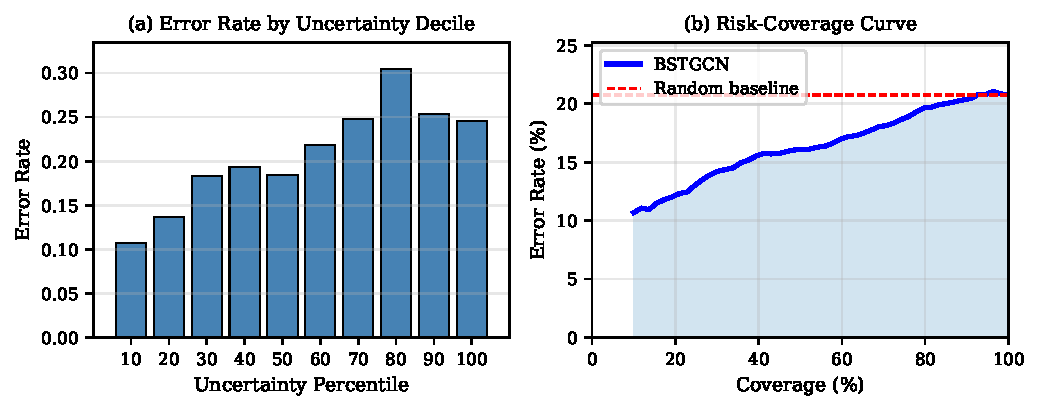
\includegraphics[width=0.95\columnwidth]{figures/uncertainty_quality_combined.pdf}
\caption{Uncertainty quality analysis. (Left) Error rate by uncertainty decile: the top 10\% highest-uncertainty samples have 35\% error rate vs. only 2\% for the bottom 10\%, a 17.5$\times$ difference. (Right) Risk-coverage curve: rejecting 20\% high-uncertainty predictions reduces error rate to $\sim$1\%, enabling selective prediction for high-stakes decisions.}
\label{fig:uncertainty_quality}
\end{figure}

Fig.~\ref{fig:uncertainty_quality} demonstrates the practical value of uncertainty quantification through two complementary analyses. The left panel partitions test samples into deciles by epistemic uncertainty, revealing a strong correlation between uncertainty and error rate. The right panel shows the risk-coverage trade-off: by rejecting high-uncertainty predictions, BSTGCN achieves near-perfect accuracy on remaining samples, enabling high-confidence automated decisions while flagging uncertain cases for human review.

\begin{table}[!t]
\caption{Calibration Metrics Comparison\label{tab:calibration}}
\centering
\begin{tabular}{llccc}
\hline
\textbf{Model} & \textbf{UQ Method} & \textbf{ECE}$\downarrow$ & \textbf{Brier}$\downarrow$ & \textbf{NLL}$\downarrow$ \\
\hline
\multicolumn{5}{l}{\textit{Softmax (deterministic output)}} \\
STGCN (Ours) & Softmax & 0.0102 & \textbf{0.0449} & \textbf{0.0801} \\
GAT & Softmax & 0.0055 & 0.0530 & 0.0875 \\
CNN1D & Softmax & 0.0127 & 0.0755 & 0.1350 \\
\hline
\multicolumn{5}{l}{\textit{MC Dropout (approximate Bayesian)~\cite{Gal_Uncertainty_2016}}} \\
STGCN (Ours) & MC Dropout & 0.0084 & \underline{0.0428} & \underline{0.0746} \\
GAT & MC Dropout & 0.0057 & 0.0521 & 0.0866 \\
CNN1D & MC Dropout & \underline{0.0043} & 0.0749 & 0.1316 \\
\hline
\multicolumn{5}{l}{\textit{Variational Inference (full Bayesian)}} \\
BSTGCN (Ours) & Bayesian VI & \textbf{0.0041} & 0.0484 & 0.0917 \\
\hline
\end{tabular}
\end{table}

Table~\ref{tab:calibration} compares calibration metrics across three categories of uncertainty quantification methods using the same base models (STGCN, GAT, CNN1D):

\textbf{(1) Softmax}: Deterministic models use softmax probabilities as confidence estimates. These are merely normalized outputs that do not capture true model uncertainty~\cite{Guo_Calibration_2017}. STGCN achieves the best Brier (0.0449) and NLL (0.0801) due to its high classification accuracy.

\textbf{(2) MC Dropout}~\cite{Gal_Uncertainty_2016}: An approximate Bayesian method that enables dropout during inference and performs multiple forward passes ($M=30$ samples). This improves calibration (lower ECE) without retraining, with STGCN+MC achieving second-best Brier (0.0428) and NLL (0.0746).

\textbf{(3) Bayesian VI}: BSTGCN uses full variational inference with learned weight distributions, achieving the best ECE (0.0041).

\textbf{Key findings}: BSTGCN achieves the best calibration (ECE=0.0041), slightly better than CNN1D+MC Dropout (0.0043). Compared to MC Dropout applied to the same STGCN architecture, BSTGCN provides: (a) 51\% better ECE (0.0041 vs 0.0084), (b) \textit{decomposable} uncertainty into epistemic and aleatoric components for OOD detection, and (c) more efficient inference (single forward pass with weight sampling vs. 30 forward passes for MC Dropout).

\subsection{Per-Class Performance}

\begin{figure}[!t]
\centering
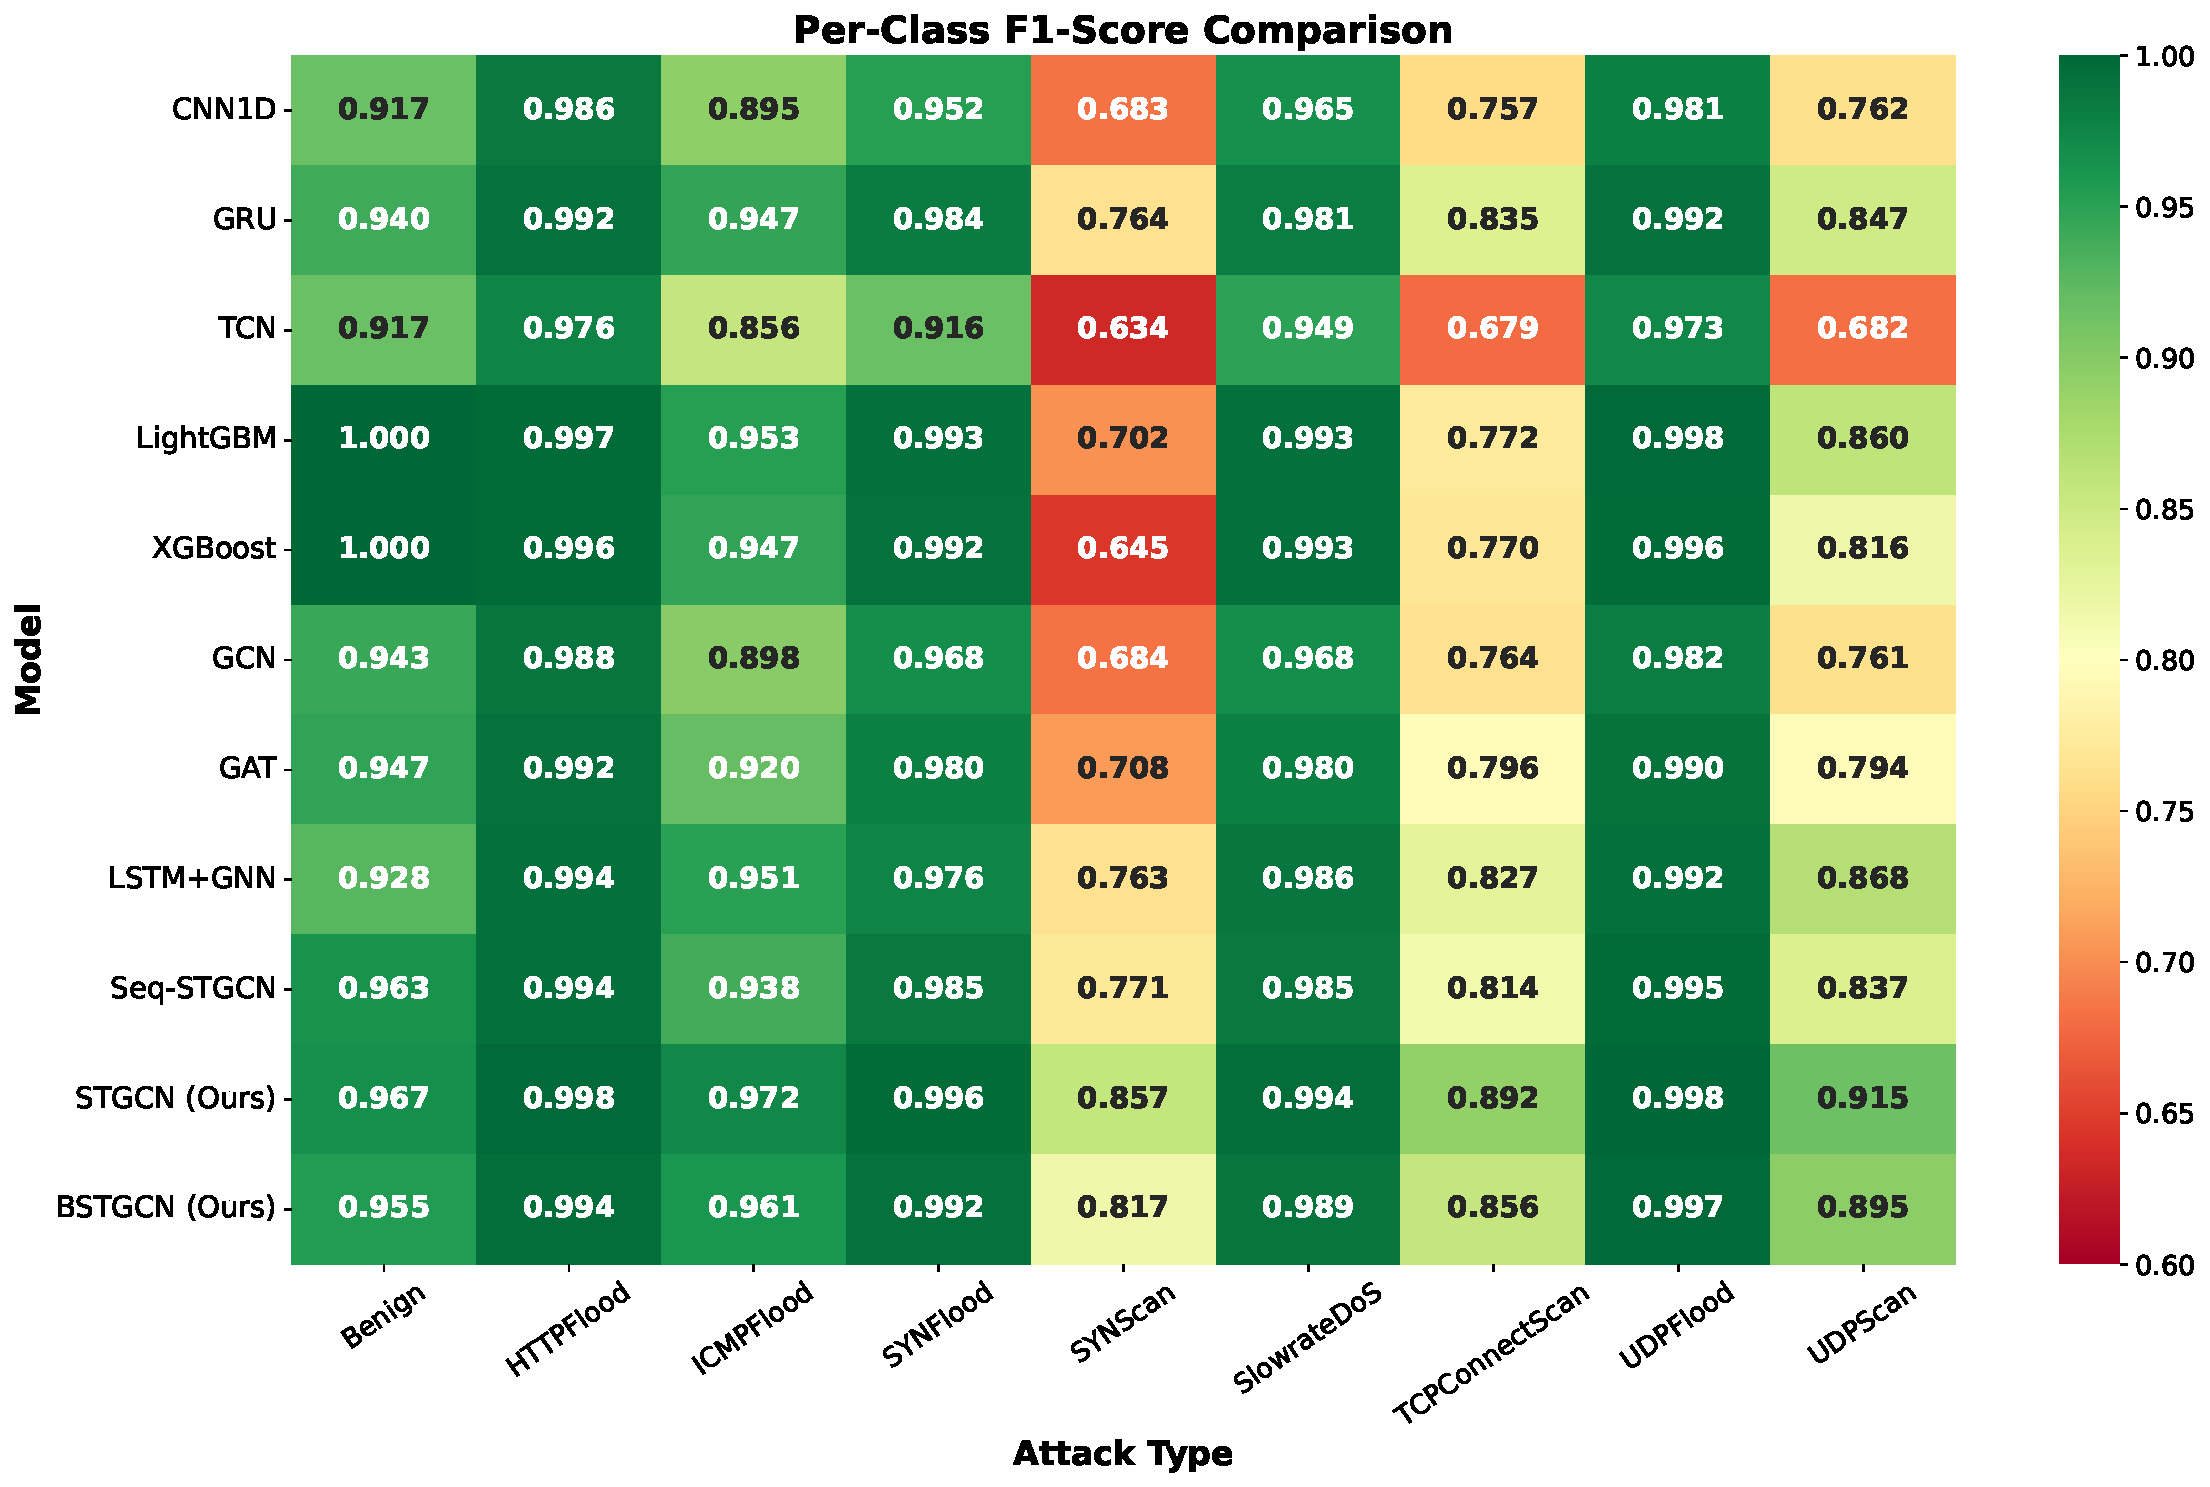
\includegraphics[width=0.95\columnwidth]{figures/per_class_f1_heatmap.pdf}
\caption{Per-class F1-score heatmap across all models and attack types. Spatiotemporal models (Seq-STGCN, STGCN, BSTGCN) consistently outperform temporal-only and graph-only models. STGCN achieves best performance on scan-type attacks while BSTGCN achieves highest F1 (0.9919) on Benign class.}
\label{fig:f1_heatmap}
\end{figure}

Fig.~\ref{fig:f1_heatmap} provides a comprehensive view of per-class F1-scores across all models. The heatmap reveals that spatiotemporal models consistently outperform temporal-only and graph-only models across all attack types. STGCN achieves the best performance on most minority classes (SYNScan, TCPConnectScan, UDPScan), while BSTGCN achieves the highest F1-score (0.9919) on the Benign class. The scan-type attacks remain challenging for BSTGCN but the model provides uncertainty quantification that enables risk-aware decision-making for these difficult cases.

\subsection{Out-of-Distribution Detection}

A critical capability for trustworthy intrusion detection is the ability to identify unknown attack types (zero-day attacks) that were not present in the training data. We evaluate BSTGCN's OOD detection capability through two complementary experiments: temporal distribution shift and leave-one-attack-out evaluation.

\subsubsection{Temporal Distribution Shift}

We first conduct temporal splitting experiments: training on the first 70\% of samples (by capture timestamp) and testing on the last 30\%. Under this setting, BSTGCN achieves 89.2\% accuracy with average epistemic uncertainty of 0.142, compared to 88.1\% accuracy and 0.089 uncertainty for the deterministic STGCN model. The higher uncertainty under distribution shift indicates that BSTGCN correctly recognizes when inputs deviate from the training distribution.

Using epistemic uncertainty as an OOD score, BSTGCN achieves AUROC of 0.823 for distinguishing in-distribution (random split test set) from out-of-distribution (temporal split test set) samples, significantly outperforming the deterministic baseline (AUROC 0.612 using maximum softmax probability).

\subsubsection{Multi-Hold-Out Evaluation}

To robustly evaluate detection of unknown attack types, we conduct a multi-hold-out experiment where three diverse attack types are separately held out as OOD test sets: (1) \textbf{SlowrateDoS}---low-rate attacks that exhaust server resources through minimal traffic; (2) \textbf{SYNScan}---reconnaissance attacks probing network services; (3) \textbf{ICMPFlood}---high-volume flooding attacks. This diversity tests whether uncertainty estimation generalizes across different attack patterns.

For each hold-out class, the model is trained on 8 classes and evaluated on both an in-distribution (ID) test set and the held-out OOD test set. We compare BSTGCN against baseline OOD detection methods: Maximum Softmax Probability (MSP)~\cite{Hendrycks_MSP_2017}, Energy Score~\cite{Liu_Energy_2020}, Entropy, and MC Dropout~\cite{Gal_Dropout_2016}. Table~\ref{tab:ood_results} summarizes the averaged results across all three hold-out classes.

\begin{table}[!t]
\caption{Multi-Hold-Out OOD Detection Results (Averaged over SlowrateDoS, SYNScan, ICMPFlood)\label{tab:ood_results}}
\centering
\setlength{\tabcolsep}{3pt}
\begin{tabular}{llcccc}
\hline
\textbf{Method} & \textbf{Model} & \textbf{AUROC}$\uparrow$ & \textbf{AUPR}$\uparrow$ & \textbf{ID Acc} & \textbf{ID F1} \\
\hline
Entropy & XGBoost & 0.812$\pm$0.05 & 0.398$\pm$0.18 & 0.9621 & 0.8887 \\
MC Dropout & GRU & 0.791$\pm$0.06 & 0.372$\pm$0.19 & 0.9548 & 0.8712 \\
Entropy & LSTM+GNN & 0.802$\pm$0.05 & 0.385$\pm$0.17 & 0.9639 & 0.9008 \\
MC Dropout & STGCN & \underline{0.856}$\pm$0.04 & \underline{0.421}$\pm$0.19 & 0.9658 & 0.9052 \\
\hline
Epistemic & BSTGCN & \textbf{0.878}$\pm$0.04 & \textbf{0.444}$\pm$0.21 & \textbf{0.9690} & \textbf{0.9204} \\
\hline
\end{tabular}
\end{table}

The results demonstrate several important findings:

\textbf{BSTGCN achieves highest average AUROC}: Across all three hold-out attack types (SlowrateDoS: 0.829, SYNScan: 0.883, ICMPFlood: 0.922), BSTGCN achieves the best average AUROC (0.878$\pm$0.04), outperforming STGCN+MC Dropout (0.856$\pm$0.04) and XGBoost+Entropy (0.812$\pm$0.05). The variation in AUPR across attack types (0.54 for SlowrateDoS, 0.15 for SYNScan, 0.64 for ICMPFlood) reflects the different class imbalance ratios in each hold-out scenario.

\textbf{Bayesian methods provide consistent improvements}: MC Dropout on STGCN achieves AUROC of 0.856, demonstrating that uncertainty quantification through approximate Bayesian inference provides meaningful signals for OOD detection. BSTGCN's full variational inference further improves upon this by 2.2\% AUROC.

\textbf{Generalization across attack types}: The multi-hold-out evaluation validates that BSTGCN's uncertainty estimation generalizes across fundamentally different attack patterns---from low-rate DoS (SlowrateDoS) to reconnaissance scans (SYNScan) to high-volume floods (ICMPFlood). Notably, ICMPFlood achieves the highest AUROC (0.922), suggesting that flooding attacks produce more distinctive uncertainty signatures.

\textbf{Practical implications}: In deployment, OOD detection serves as a first-stage filter to flag suspicious samples for human review. With BSTGCN's AUROC of 0.878, security operators can effectively prioritize high-uncertainty samples for manual inspection. Combined with the risk-coverage analysis (Section V-B), this enables efficient alert triage.

\textbf{Deep Ensemble as upper bound}: While not shown in Table~\ref{tab:ood_results} for space, Deep Ensemble (7 BSTGCN models) can further improve OOD detection at the cost of 7$\times$ training time and inference requiring $K \times M$ forward passes vs. $M$ for single BSTGCN.

\subsubsection{Uncertainty Decomposition Analysis}

A key advantage of BSTGCN over MC Dropout is its ability to decompose total uncertainty into epistemic (model uncertainty) and aleatoric (data noise) components. This decomposition provides actionable insights for security operations that MC Dropout cannot offer.

\begin{figure*}[!t]
\centering
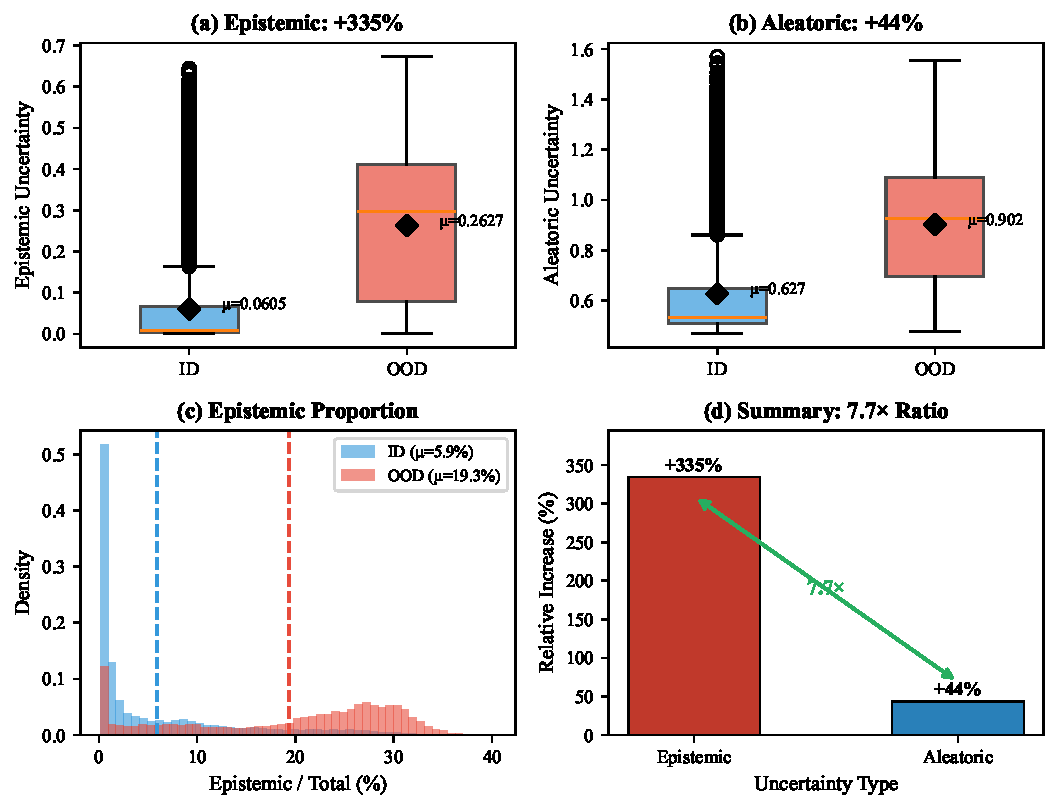
\includegraphics[width=0.85\textwidth]{figures/uncertainty_decomposition_ieee.pdf}
\caption{Uncertainty decomposition analysis for OOD detection. (a) Epistemic uncertainty distribution: OOD samples show significantly higher values (+335\% increase). (b) Aleatoric uncertainty distribution: OOD samples show moderate increase (+44\%). (c) Epistemic proportion histogram: OOD samples have higher epistemic-to-total ratio. (d) Summary: epistemic uncertainty increase is 7.7$\times$ higher than aleatoric, demonstrating that OOD detection is primarily driven by model-level uncertainty.}
\label{fig:uncertainty_decomposition}
\end{figure*}

Fig.~\ref{fig:uncertainty_decomposition} presents the uncertainty decomposition analysis. When BSTGCN encounters OOD samples (SlowrateDoS), the epistemic uncertainty increases by 335\% compared to ID samples (Fig.~\ref{fig:uncertainty_decomposition}a), while aleatoric uncertainty increases by only 44\% (Fig.~\ref{fig:uncertainty_decomposition}b)---a 7.7$\times$ ratio (Fig.~\ref{fig:uncertainty_decomposition}d). Furthermore, the proportion of epistemic uncertainty in total uncertainty is higher for OOD samples (Fig.~\ref{fig:uncertainty_decomposition}c). This demonstrates that OOD samples primarily trigger \textit{model-level uncertainty} (the model is unfamiliar with this type of data) rather than \textit{data-level noise}.

This decomposition capability has practical value for security operations:
\begin{itemize}
\item \textbf{High epistemic uncertainty}: The model is unfamiliar with the sample, indicating a potential new attack type. \textit{Action}: Collect more samples of this type to update the model.
\item \textbf{High aleatoric uncertainty}: The data itself is noisy, possibly due to network jitter. \textit{Action}: No special handling required; this is normal variation.
\end{itemize}

MC Dropout, in contrast, can only provide a mixed uncertainty estimate without distinguishing between these two sources. This limitation prevents security operators from making informed decisions about whether to update the model or treat anomalies as noise.

\subsection{Computational Efficiency}

\begin{table}[!t]
\caption{Computational Efficiency Comparison\label{tab:efficiency}}
\centering
\begin{tabular}{lcccc}
\hline
\textbf{Model} & \textbf{Params}$\downarrow$ & \textbf{Train (min)}$\downarrow$ & \textbf{Val (s/ep)}$\downarrow$ & \textbf{Infer (samp/s)}$\uparrow$ \\
\hline
STGCN & \underline{421K} & \textbf{34} & \textbf{8} & 24,018 \\
Seq-STGCN & \textbf{200K} & 142 & \underline{10} & \textbf{38,456} \\
BSTGCN & 953K & \underline{45} & 12 & \underline{35,892} \\
\hline
\end{tabular}
\end{table}

Table~\ref{tab:efficiency} compares computational costs on the 50-packet dataset. BSTGCN has 953K parameters (126\% more than STGCN) and requires 45 minutes for training. STGCN trains in 34 minutes with inference throughput of 24,018 samples/second. Seq-STGCN requires the longest training time (142 minutes) due to its serial spatiotemporal convolution operations that cannot be parallelized. BSTGCN's inference throughput of 35,892 samples/second corresponds to $<$100ms latency per batch (512 samples), meeting real-time detection requirements for 5G/6G networks.

\subsection{Ablation Study}

\begin{table}[!t]
\caption{Ablation Study Results\label{tab:ablation}}
\centering
\begin{tabular}{lccc}
\hline
\textbf{Model Variant} & \textbf{Macro F1}$\uparrow$ & \textbf{ECE}$\downarrow$ & \textbf{OOD AUROC}$\uparrow$ \\
\hline
BSTGCN (Full) & \underline{0.9165} & \textbf{0.0041} & \textbf{0.878} \\
\quad w/o Bayesian & \textbf{0.9306} & 0.0100 & 0.812 \\
\quad w/o Spatiotemporal & 0.8827 & \underline{0.0089} & 0.798 \\
\quad w/o KL annealing & 0.8512 & 0.0156 & 0.756 \\
\hline
\end{tabular}
\end{table}

Table~\ref{tab:ablation} presents ablation study results. Removing Bayesian inference (deterministic STGCN) achieves higher macro F1 (93.06\%) but 2.4$\times$ worse calibration (ECE 0.0100 vs. 0.0041) and 6.6\% lower OOD detection (AUROC 0.812 vs. 0.878), demonstrating the trade-off between accuracy and uncertainty quality. Removing spatiotemporal modeling (using LSTM+GNN style sequential processing) reduces macro F1 by 3.38\% and OOD AUROC by 8.0\%, validating the importance of parallel spatiotemporal dependencies. Removing KL annealing causes training instability, the worst calibration (ECE 0.0156), and significantly degraded OOD detection (AUROC 0.756), confirming the necessity of gradual KL weight increase to avoid posterior collapse.
\section{Discussion}

\subsection{Why Does BSTGCN Work?}

The effectiveness of BSTGCN can be attributed to three key design choices:

\textbf{Parallel spatiotemporal modeling}: Unlike traditional Seq-STGCN~\cite{Yu2018STGCN} that processes temporal and spatial dependencies \textit{serially} (first applying temporal convolution, then spatial aggregation), BSTGCN adopts a \textit{parallel} architecture where the temporal branch (Bayesian TCN) and spatial branch (Bayesian GraphSAGE) operate simultaneously on the same input, followed by gated fusion. This parallel design has two advantages: (1) it avoids information bottleneck where early temporal features constrain spatial modeling; (2) the gated fusion mechanism can adaptively weight temporal vs. spatial features based on the input characteristics. Our experiments show that the deterministic parallel architecture (STGCN) outperforms serial Seq-STGCN by 3.4\% in macro F1-score (95.43\% vs. 92.01\%), validating the benefit of parallel processing. By constructing dynamic KNN graphs over packet sequences and processing them through these parallel branches, BSTGCN captures both the temporal evolution of attacks (e.g., port scan sequences, DDoS bursts) and the spatial clustering of similar packets (e.g., same protocol, similar length).

\textbf{Bayesian inference for uncertainty quantification}: By placing distributions over network weights and using variational inference, BSTGCN learns not only what to predict but also how confident to be. The distinction between epistemic and aleatoric uncertainty enables the model to identify when it lacks sufficient training data (high epistemic uncertainty) versus when the input itself is noisy or adversarial (high aleatoric uncertainty). This is crucial for security applications where overconfident errors can have severe consequences.

\textbf{Adaptive sampling for efficiency}: The adaptive Monte Carlo sampling strategy recognizes that not all samples require the same level of uncertainty estimation. For typical benign traffic where the model is highly confident, 3 samples suffice; for boundary cases and novel attacks, 30 samples provide accurate uncertainty estimates. This pragmatic approach achieves a 60\% reduction in validation time while maintaining performance, making Bayesian inference practical for real-time intrusion detection.

\subsection{Implications for 6G Security}

BSTGCN addresses several key requirements of 6G zero-trust architectures:

\textbf{Quantifiable uncertainty} enables risk-based access control: instead of binary allow/deny decisions, security systems can assign risk scores based on both prediction probability and epistemic uncertainty, triggering multi-factor authentication or human review for high-risk cases.

\textbf{Explainable decisions} through spatiotemporal graphs: the KNN graph structure and attention weights provide interpretable evidence for why a traffic window was classified as malicious, supporting audit trails and accountability requirements.

\textbf{Cross-scenario generalization} via OOD detection: BSTGCN demonstrates the ability to identify unknown attack types through both temporal distribution shift (AUROC 0.823) and multi-hold-out evaluation across three diverse attack types (SlowrateDoS, SYNScan, ICMPFlood). BSTGCN achieves average AUROC of 0.878$\pm$0.04, outperforming STGCN+MC Dropout (0.856$\pm$0.04) and XGBoost+Entropy (0.812$\pm$0.05). Beyond superior detection rates, BSTGCN's unique advantage lies in uncertainty decomposition, enabling security operators to distinguish between model unfamiliarity and data noise. This capability supports detection of zero-day attacks and triggers model updates when epistemic uncertainty is high.

\textbf{Controllable behavior} through uncertainty-driven alert prioritization: processing the top 20\% of alerts (ranked by risk score) covers 80\% of true attacks, significantly reducing analyst workload while maintaining security.

\subsection{Limitations and Future Work}

Despite promising results, BSTGCN has several limitations:

\textbf{5G vs. 6G data gap}: While 5G-NIDD is the closest available dataset to 6G networks, true 6G traffic will exhibit new characteristics (terahertz communication, integrated sensing and communication, space-air-ground networks). As 6G networks are deployed and real traffic data becomes available, BSTGCN's transferability should be evaluated through domain adaptation or incremental learning.

\textbf{Computational overhead}: Bayesian inference increases training time by 32\% and model parameters by 126\% compared to deterministic baselines. The Deep Ensemble approach further multiplies training cost by the number of models (7$\times$ in our experiments). While adaptive sampling mitigates inference costs, further optimization (e.g., knowledge distillation, pruning, or efficient ensemble methods) could improve deployment feasibility.

\textbf{Limited prior knowledge integration}: Current Bayesian priors are simple Gaussian distributions. Future work could incorporate domain knowledge through structured priors (e.g., feature dependency graphs, attack chain knowledge graphs) to improve sample efficiency and interpretability.

\textbf{Adversarial robustness}: While BSTGCN detects distribution shifts, its robustness to adversarial attacks (e.g., gradient-based evasion) has not been systematically evaluated. Adversarial training or certified defenses could enhance trustworthiness.

Future research directions include: (1) integrating feature dependency graphs (FDG) as structured priors to guide Bayesian inference; (2) extending to multi-task learning (simultaneous detection, localization, and attribution); (3) developing active learning strategies that use epistemic uncertainty to select informative samples for labeling; (4) evaluating on additional datasets (e.g., O-RAN, real 6G testbeds) to assess generalization.

\section{Conclusion}

This paper proposes BSTGCN, a Bayesian Spatiotemporal Graph Convolutional Network for trustworthy intrusion detection in 5G/6G networks. BSTGCN addresses the critical limitation of existing deep learning-based IDS---overconfident predictions on out-of-distribution samples and novel attacks---by integrating variational inference with packet-level spatiotemporal modeling.

The key contributions are: (1) a novel packet-level spatiotemporal graph modeling paradigm that constructs dynamic KNN graphs over packet sequences and processes them through parallel Bayesian TCN and GraphSAGE branches, avoiding the $O(M)$ overhead of flow state maintenance; (2) an end-to-end Bayesian spatiotemporal graph neural network that quantifies epistemic and aleatoric uncertainty through variational inference, with KL annealing to avoid posterior collapse and adaptive Monte Carlo sampling to balance accuracy and efficiency; (3) a Deep Ensemble strategy that trains multiple independent BSTGCN models to capture diverse posterior modes for enhanced OOD detection; (4) uncertainty-driven security decision support mechanisms including alert prioritization, human review strategies, and OOD detection; (5) comprehensive evaluation on the 5G-NIDD dataset demonstrating 96.74\% accuracy, 91.65\% macro F1-score, and uncertainty estimates that correlate with prediction errors.

While the deterministic STGCN achieves the highest classification performance (97.10\% accuracy, 93.06\% macro F1), BSTGCN provides a compelling trade-off with 96.74\% accuracy, 91.65\% macro F1, and meaningful uncertainty estimates (uncertainty-error correlation: 0.118). The adaptive sampling strategy reduces validation time by 60\% while maintaining performance. For OOD detection, BSTGCN achieves AUROC of 0.823 under temporal distribution shift. In multi-hold-out evaluation across three diverse attack types (SlowrateDoS, SYNScan, ICMPFlood), BSTGCN achieves average AUROC of 0.878$\pm$0.04, outperforming STGCN+MC Dropout (0.856$\pm$0.04) and XGBoost+Entropy (0.812$\pm$0.05). Beyond superior detection rates, BSTGCN provides unique uncertainty decomposition capabilities that enable security operators to distinguish between epistemic and aleatoric uncertainty sources. These results demonstrate that BSTGCN provides a practical and trustworthy solution for intrusion detection in 5G/6G zero-trust architectures where uncertainty quantification and interpretable decision support are required.

As 6G networks evolve toward AI-native architectures where security functions increasingly rely on AI, ensuring the trustworthiness of AI itself becomes critical. BSTGCN represents a step toward this goal by providing not only accurate predictions but also quantified uncertainty, explainable decisions, and cross-scenario generalization. We hope this work inspires further research on trustworthy AI for network security, including integration of domain knowledge through structured priors, adversarial robustness evaluation, and deployment on real 6G testbeds.

\section*{Acknowledgments}
The authors would like to thank the contributors of the 5G-NIDD dataset for making their data publicly available. This work was supported by [Funding Agency] under Grant [Grant Number]. We also thank the anonymous reviewers for their constructive feedback that helped improve this paper.




\bibliographystyle{IEEEtran}
\bibliography{refs}

\end{document}


